\chapter{Vorlesung}
\subsection*{Dijkstra Algorithmus (Fortsetzung)}
\[ G=(V,E)~~ w:E\rightarrow \mathbb{R}^{\geq0} \]
\begin{wrapfigure}{R}{0.3\textwidth}
	\centering
	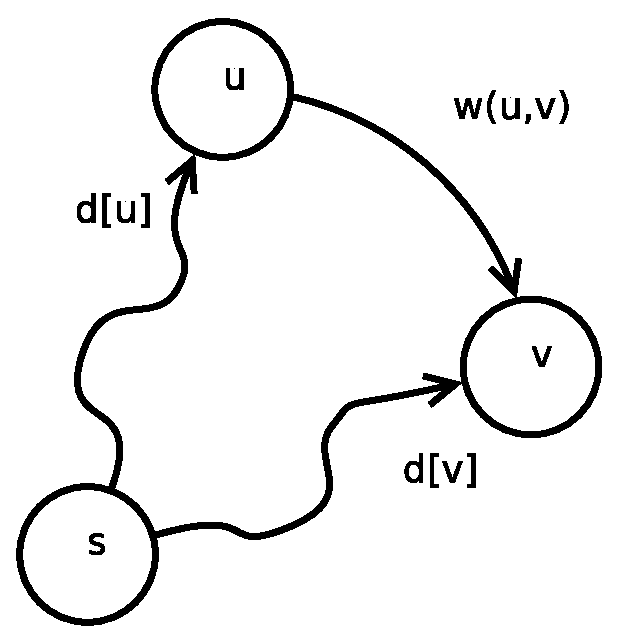
\includegraphics[width=\linewidth]{17/Grafik/Skizze}
	\caption{}
	\label{fig:Skizze}
\end{wrapfigure}
\begin{lstlisting}
forall (v /eIn V) {
  d[v] = /inf;
  /pi[v] = NULL;
}
d[s] = 0;
S = /leer;
PriorityQueue PQ;
forall (v /eIn V)
  PQ.insert((d[v],v));
while(!PQ.empty()) {
  u = PQ.deleteMin();
  forall( (u,v) /eIn E) {
    if ( d[v] > d[u] + w(u,v)) {
      d[v] = d[u] + w(u,v);
      /pi[v] = u;
      PQ.decreaseKey((d[v],v));
    }
  }
  S = S/cup{u};
}
\end{lstlisting}

\paragraph{Satz:}
Der Dijkstra Algorithmus berechnet alle d-Werte, so dass nach Ablauf des Algo $\forall~v\in V$ gilt: $d[v] = \delta(s,v)$.
\pagebreak
\paragraph{Beweis:}
\subparagraph{Annahme:}
\[ \exists v\in V:~d[v]\neq\delta(s,v) \]
\[ \overset{Lemma Relax}{\Longrightarrow}~d[v]>\delta(s,v) \]
\begin{wrapfigure}{r}{0.3\textwidth}
	\vspace{-80pt}
	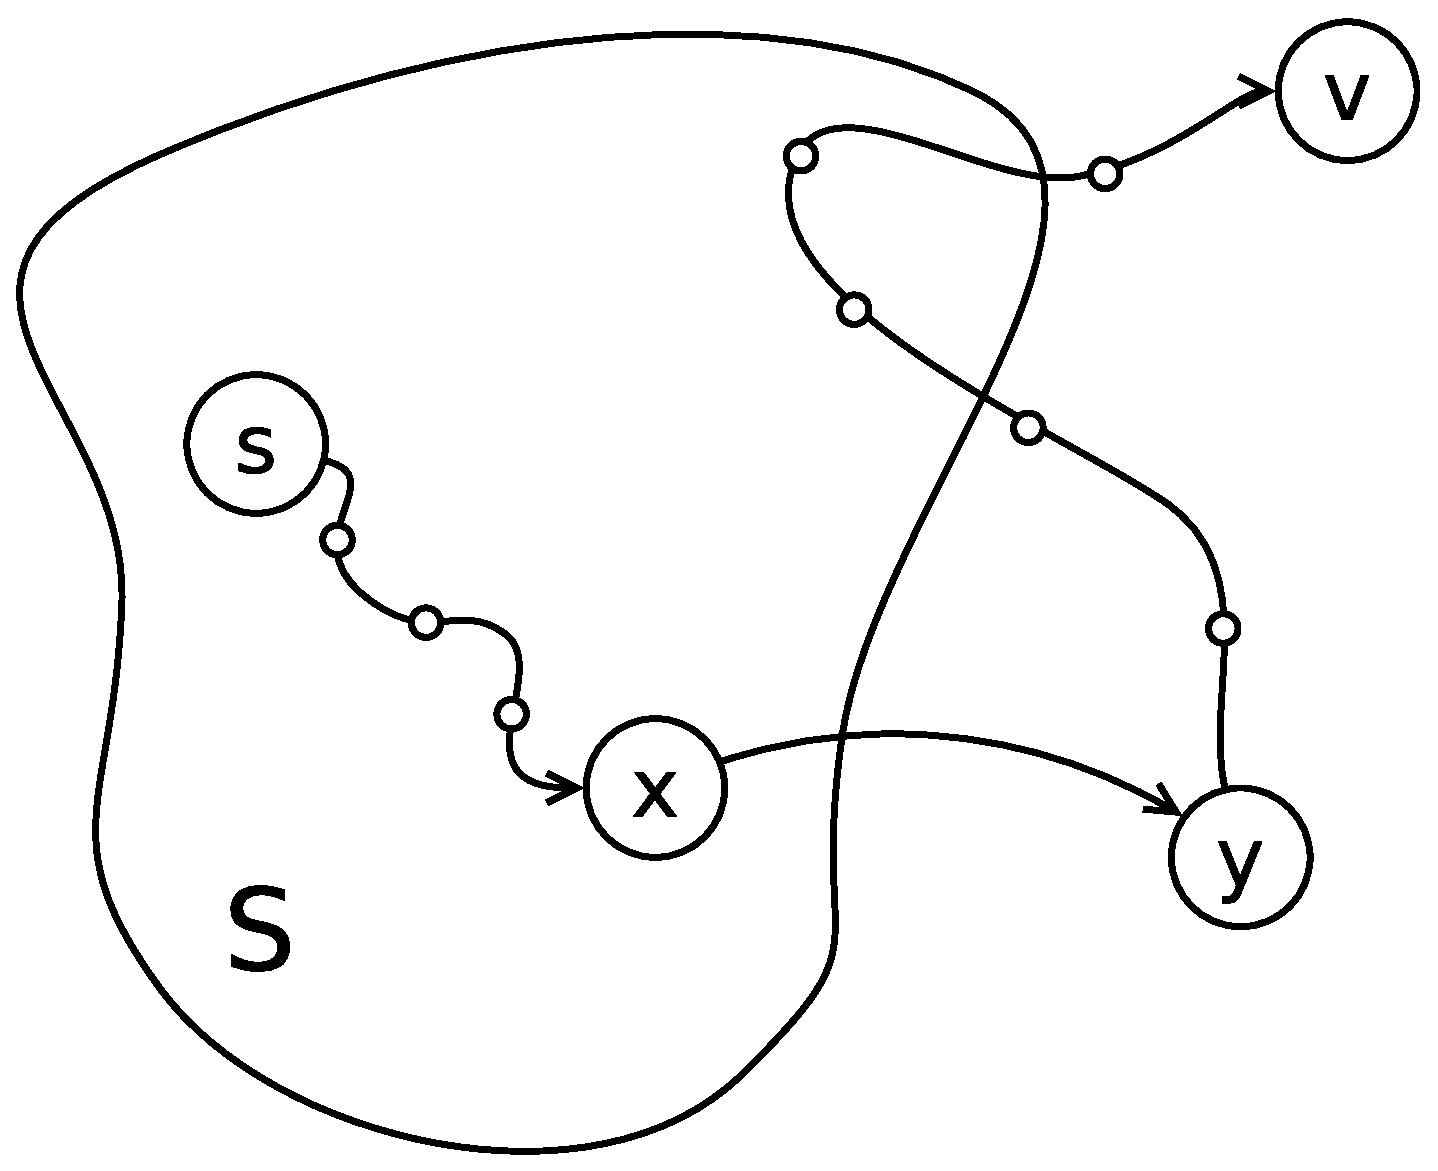
\includegraphics[width=\linewidth]{17/Grafik/Skizze2}
	\caption{Skizze}
	\label{fig:Skizze2}
\end{wrapfigure}
Sei $v$ so gewählt, das $v$ der erste Knoten mit der Eigenschaft ist, der mit \textrm{deleteMin} der \textrm{PQ} entnommen wird und nach Relaxation aller von ihm ausgehenden Kanten der Menge S hinzugefügt wird.

Betrachte einen kürzesten Weg $s \rightsquigarrow v$
\[ d[v] > \delta(s,v) \geq\footnote{weil Kantengewichte nicht negativ sein dürfen}\delta(s,y)=d[y]=\footnote{x wurde schon zu S hinzugefügt, hat also Korrekten d-Wert $d[x] 
	= \delta(s,x)$}d[x]+w(x,y)=d[y]\geq\footnote{weil v vor y aus der PQ entnommen wird.} d[v] ~~\lightning \]
\subsection{Vorläufige Laufzeitanalyse von Dijkstra}
\begin{tabular}{ccc}
	\textrm{PQ.insert} & x & $|V|$ \\
	\textrm{PQ.empty} & x & $|V|$ \\
	\textrm{PQ.deleteMin} & x & $|V|$ \\
	\textrm{PQ.decreaseKey} & x & $|E|$ 
\end{tabular}
Mit balanciertem Suchbaum oder mit binärem Heap (siehe Heapsort) %Link setzen
können diese Opeartionen alle in Zeit $\mathcal{O}(\log|V|)$ realisiert werden.\\
$\Rightarrow$ Gesamtlaufzeit: $\mathcal{O}((|V|+|E|)\log|V|)$\\
Wir werden später zeigen, dass Laufzeit $\mathcal{O}(|V|\log|V|+|E|)$ möglich ist.
\section{Bellman-Ford-Algorithmus}
\[ G=(V,E)~~w:~E\rightarrow \mathbb{R} \]
\paragraph{Voraussetzung}
$G$ enthält keine negativen Zyklen
\begin{figure}[h]
\centering
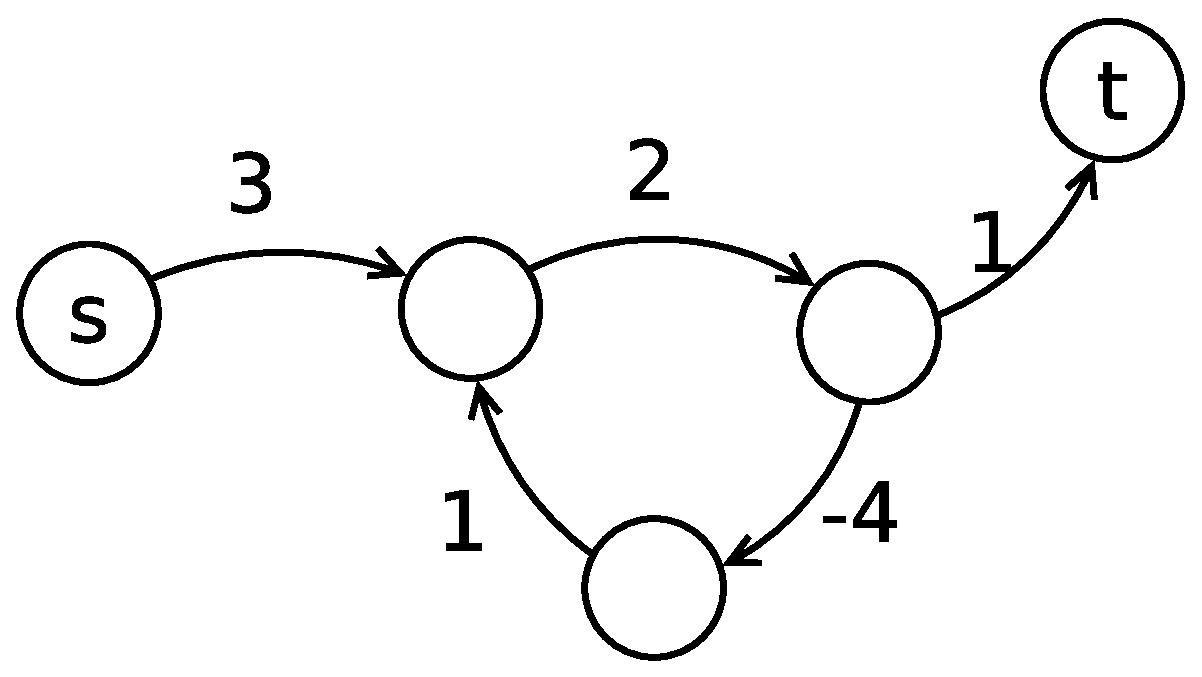
\includegraphics[width=0.7\linewidth]{17/Grafik/Skizze3}
\caption{Ein verbotener, negativer Zyklus}
\label{fig:Skizze3}
\end{figure}
\subsection{Pseudocode}
\begin{lstlisting}
forall(v /eIn V) {
  d[v] = /inf;
  /pi[v] = NULL;
}
d[s] = 0;
for(i = 1; i < |V|; i++ )
  forall((u,v) /eIn E)
    if( d[v] > d[u] + w(u,v)) {
      d[v] = d[u] + w(u,v);
      /pi[v] = u;
    }
\end{lstlisting}
\subsection{Laufzeit: Bellman-Ford}
\[ \mathcal{O}(|V|\cdot|E|) \]
\subsection{Korrektheitsbeweis: Bellman-Ford}
\paragraph{Invariante:}
Nach den $i$-ten Schleifendurchlauf sind alle Kürzesten Wege korrekt berechnet, die $\leq i$ Kanten benutzen.
\paragraph{Beweis: Induktion über i}
\subparagraph{Induktionsanfang}
\begin{description}
	\item[$i=0$] $d[s] = 0 = \delta(s,s)$, da keine negativen Zyklen vorliegen.
\end{description}
\subsection{Induktionsschritt:  $i\rightarrow i+1$}
Betrachte kürzesten Weg mit $i+1$ Kanten:
\[ s=v_0\rightarrow v_1\rightarrow v_2\rightarrow\ldots\rightarrow v_i\rightarrow v_{i+1} \]
Aufgrund der Induktionsannahme\footnote{Die Invariante} gilt: $d[v_i] = \delta(s,v_i)$, weil $s=v_0\rightarrow v_1\rightarrow\ldots\rightarrow v_i$ ein kürzester Weg $s\rightsquigarrow v_i$ mit $i$ Kanten ist.
Da alle Kanten in der inneren Schleife einmal relaxiert werden, trifft dies insbesondere auf die Kante $(v_i, v_{i+1})$ zu:
\[ d[v_{i+1}] = d[v_i] + w(v_i, v_{i+1}) = \delta(s, v_i) + w(v_i, v_{i+1}) = \delta(s,v_{i+1}) \]
\paragraph{Frage:}
Warum folgt aus der Gültigkeit dieser Invariante die Korrektheit des Algo?
\paragraph{Antwort}
Alle kürzesten Wege benutzen höchstens $|V|-1$ Kanten, ansonsten hätten sie einen Zyklus mit Gewicht $\geq 0$, den man auch weglassen kann.
\begin{lstlisting}
//Erkennung der Existenz negativer Zyklen
forall((u,v) /eIn E)
  if(d[v] > d[u] + w(u,v))
    negativer Zyklus
\end{lstlisting}